\chapter{Exceptions}
\label{sec:exceptions}
An exception is a fairly generic term for an event which occurs which the CPU needs to deal with in some way. Examples of exceptions would be the microcontroller resetting or the CPU attempting to access invalid memory or a peripheral generating an interrupt. Typically we write a block of instruction which we want to execute when an exception occurs. That block of code is called an \emph{exception handler}. We then place the address of the start of that exception handler into a special location in memory called a vector. Each exception has a vector address associated with it. The block of all vectors is called the vector table. A summarised version of it is shown in \autoref{fig:vector_table_summarised}.

\begin{figure}
\centering
\includegraphics[page=23, clip=true, trim=60 476 68 168, width=\textwidth]{./stm32f0xx_programming_manual}
% left, bottom, right, top
\caption{Summarised version of the vector table showing the CPU exceptions only. Source: Table 12, Programming Manual}
\label{fig:vector_table_summarised}
\end{figure}

When an exception occurs, the CPU performs a few tasks in order to service the exception:
\begin{itemize}
    \item Save the current 'system state' to the stack in the form of a stack frame. This is basically just pushing a few important registers to the stack. The exact format of the stack frame is shown in \autoref{fig:stack_frame}.
    \item Fetch the data from the vector associated with that exception that occurred and load that data into the PC.
    \item Start executing the block of instructions pointed to by the vector
\end{itemize}

Following is a discussion on some of the key exceptions.

\begin{figure}
\centering
\includegraphics[page=26, clip=true, trim=135 315 100 410, width=\textwidth]{./stm32f0xx_programming_manual}
% left, bottom, right, top
\caption{Stack frame. These registers are push to the stack thereby saving their state when an exception occurs. Source: Figure 9, Programming Manual}
\label{fig:stack_frame}
\end{figure}

\section{Reset}
There are a number of possible causes of a reset all detailed in section 7.1.2 of the Reference Manual. They key ones are a power reset where the power to the micro is cycles or a NRST pin reset where the Negative ReSeT pin is pulled low and then released. 

When this exception occurs the microcontroller:
\begin{itemize}
    \item aborts execution of code, 
    \item sets all registers to their default values,
    \item fetches the data from the reset vector,
    \item places that data into the PC and starts execution. 
\end{itemize}

The reset exception is fairly specialised in that is the only exception which does not cause the previous system state to be stacked. Quite the opposite in fact, it clears all state and begins fresh. 

\section{HardFault}
A HardFault occurs when an instruction attempts to do something illegal or a peripheral attempts to do an illegal memory transfer. This includes attempting to access unimplemented memory addresses or trying to perform unaligned memory access or trying to execute an instruction which has a non-existent opcode. The full list of events which cause a HardFault exception are detailed in Table B1-6 of the ARMv6-M Architecture Reference Manual.

Typically HardFaults are unrecoverable: when a HardFault happens there is generally something broken in the code and we do not want the code to carry on running. Rather we want to be made aware of the issue so that the code can be corrected. 

When a HardFault happens the standard exception handling procedure takes place: the current state is stacked, the exception handler vector is fetched an executed. Due to the fact that the state is saved on the stack it is possible to return from the handler and resume execution of the main code but it would be unusual to want to do this due to the severity of a HardFault.


%\begin{overpic}[grid,page=23]{./stm32f0xx_programming_manual}
%\end{overpic}
